%%%%%%%%%%%%%%%%%%%%%%%%%%%%%%%%%%%%%%%%%
% Developer CV
% LaTeX Template
% Version 1.0 (28/1/19)
%
% This template originates from:
% http://www.LaTeXTemplates.com
%
% Authors:
% Jan Vorisek (jan@vorisek.me)
% Based on a template by Jan Küster (info@jankuester.com)
% Modified for LaTeX Templates by Vel (vel@LaTeXTemplates.com)
%
% License:
% The MIT License (see included LICENSE file)
%
%%%%%%%%%%%%%%%%%%%%%%%%%%%%%%%%%%%%%%%%%

%----------------------------------------------------------------------------------------
%	PACKAGES AND OTHER DOCUMENT CONFIGURATIONS
%----------------------------------------------------------------------------------------

\documentclass[9pt]{developercv} % Default font size, values from 8-12pt are recommended

%----------------------------------------------------------------------------------------

\begin{document}

%----------------------------------------------------------------------------------------
%	TITLE AND CONTACT INFORMATION
%----------------------------------------------------------------------------------------

\begin{minipage}[t]{0.14\textwidth} % 45% of the page width for name
	\vspace{-\baselineskip} % Required for vertically aligning minipages
	
	% If your name is very short, use just one of the lines below
	% If your name is very long, reduce the font size or make the minipage wider and reduce the others proportionately
%\colorbox{black}{{\huge\textcolor{white}{\textbf{\MakeUppercase{Cesar Ochoa}}}}} % First name
\begin{tikzpicture}
    \clip (-0.5,-1.75) rectangle +(2.1cm,2.1cm);
    
    \node at (0,-.75) {\includegraphics[width = 3cm]{img/scotland_far.JPG}};
    %\clip (-1.5,-2.4) rectangle +(2cm,2cm);
    
    %\node at (0,-.75) {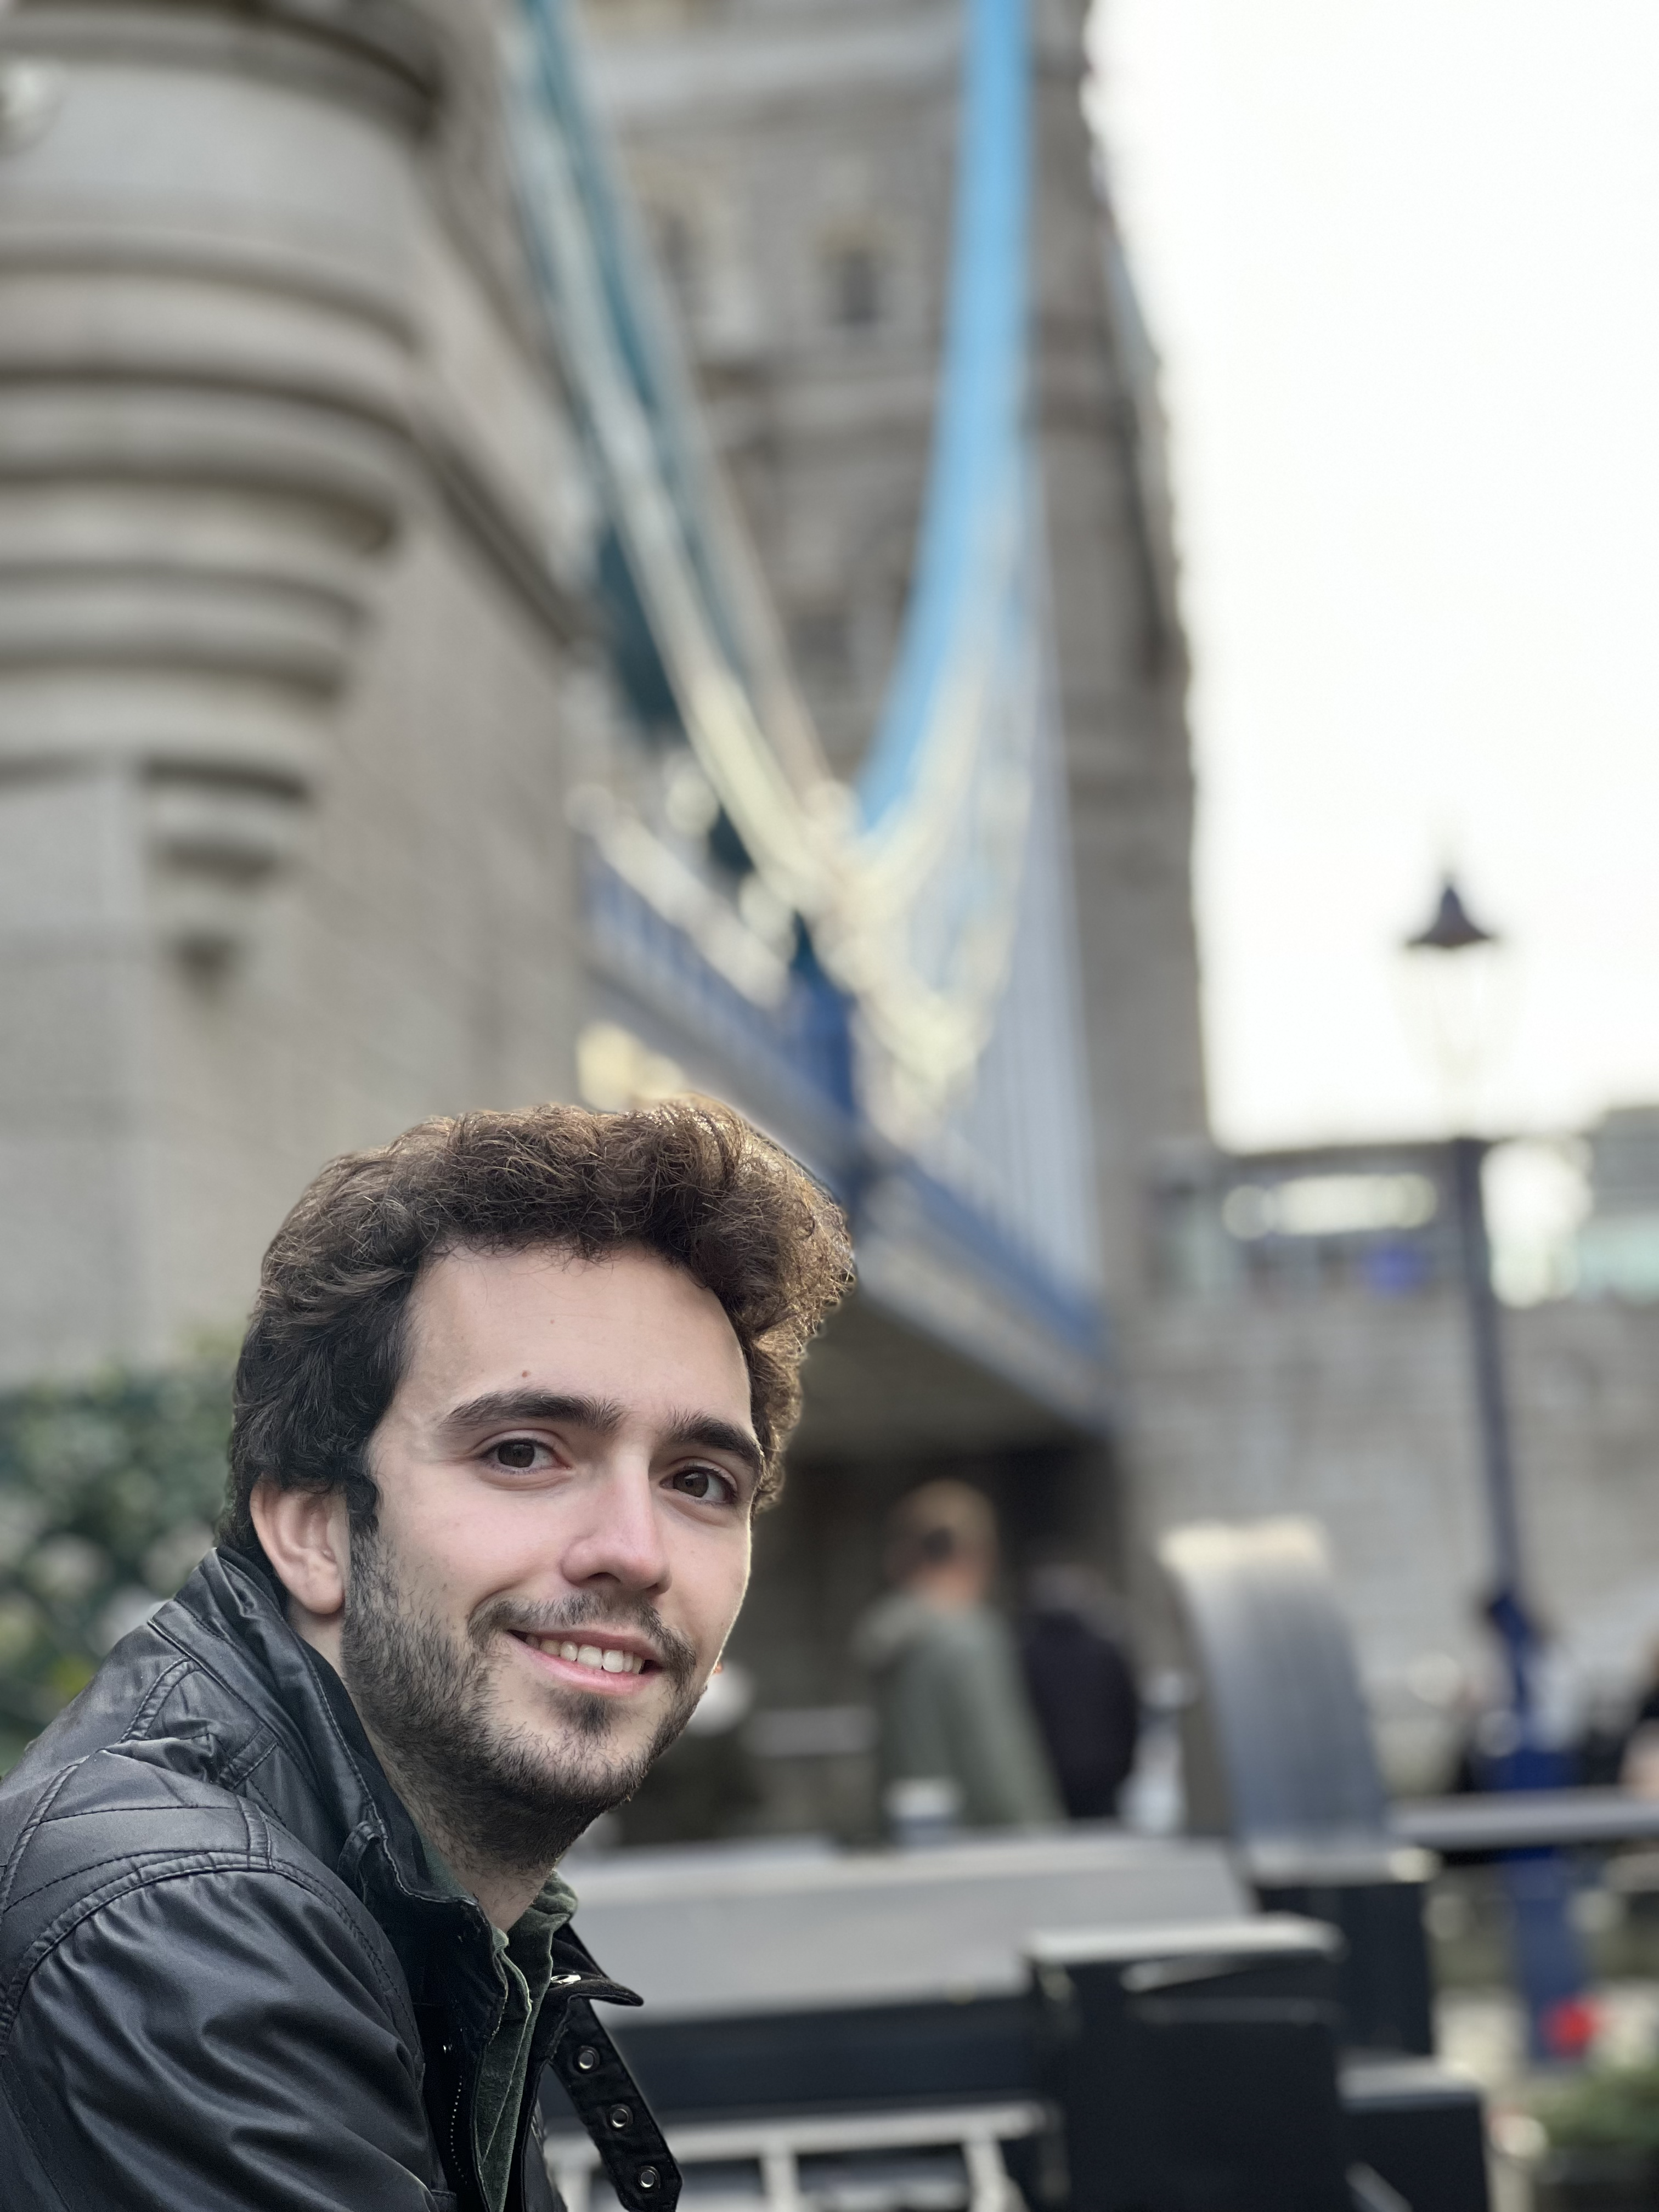
\includegraphics[width = 3cm]{img/london.png}};
    % if necessary the picture may be moved by changing the at (coordinates)
    % width defines the 'zoom' of the picture
\end{tikzpicture}
\end{minipage}
\begin{minipage}[t]{0.56\textwidth} % 45% of the page width for name
	\vspace{-\baselineskip}
	\fontsize{21}{26}{\textbf{César Ochoa Munárriz}}% First name
	
%	\colorbox{black}{{\textcolor{white}{\textbf{\MakeUppercase{Ochoa}}}}} % Last name
	
	\vspace{6pt}
	
	\large \textbf{Ingeniero de IA}, Grupo Oesía\\
 \textbf{MSc Design Informatics}, The University of Edinburgh\\
\textbf{BSc Mathematics}, The University of Manchester% Career or current job title
\end{minipage}
\begin{minipage}[t]{0.30\textwidth} % 27.5% of the page width for the first row of icons
	\vspace{-\baselineskip} % Required for vertically aligning minipages
	\begin{flushright}
	\vspace{5pt}
	% The first parameter is the FontAwesome icon name, the second is the box size and the third is the text
	% Other icons can be found by referring to fontawesome.pdf (supplied with the template) and using the word after \fa in the command for the icon you want
	
	%\icon{MapMarker}{12}{Flat 48, 117 Hornsey Lane, London, N6 5NW}\\
	\icon{Phone}{12}{+34 636 382 118}\\
	\icon{At}{12}{\href{mailto:caeochoa@gmail.com}{caeochoa@gmail.com}}\\
    \icon{Linkedin}{12}{\href{https://www.linkedin.com/in/caeochoa/}{/in/caeochoa}}\\
    
   % \large{Manchester}\\
    %\large{+44 (0) 792 393 6908}\\
    %\large{caeochoa@gmail.com}\\
    \end{flushright}
\end{minipage}
%\begin{minipage}[t]{0.275\textwidth} % 27.5% of the page width for the second row of icons
%	\vspace{-\baselineskip} % Required for vertically aligning minipages
	
	% The first parameter is the FontAwesome icon name, the second is the box size and the third is the text
	% Other icons can be found by referring to fontawesome.pdf (supplied with the template) and using the word after \fa in the command for the icon you want
%	\icon{Linkedin}{12}{\href{https://www.linkedin.com/in/caeochoa/}{/in/caeochoa}}\\
%\end{minipage}

\vspace{0.5cm}

%----------------------------------------------------------------------------------------
%	INTRODUCTION, SKILLS AND TECHNOLOGIES
%----------------------------------------------------------------------------------------
%----------------------------------------------------------------------------------------
%	EXPERIENCE
%----------------------------------------------------------------------------------------
%----------------------------------------------------------------------------------------
%	add list of skills as tags, highlighting the most relevant ones for each job?
%----------------------------------------------------------------------------------------


\cvsect{Experiencia laboral}

\begin{entrylist}
	
\bentry
{2024 -- presente}
{Ingeniero de IA}
{Grupo Oesía}
{\begin{itemize}
    \item{Desarrollo del backend de OKM, una plataforma de Inteligencia Artifical Generativa para em-
presas. Implementación de agentes de IA con funcionalidades de preguntas y respuestas sobre
documentos, traducción de consultas SQL y razonamiento en varios pasos con capacidades de
auto-validación}
\end{itemize}

\texttt{Python}\slashsep\texttt{LangChain}\slashsep\texttt{PyTorch}\slashsep\texttt{Azure}\slashsep\texttt{SQL}}
            
\bentry
{2022 -- 2024}
{Technical Business Analyst}
{Acturis}
{\begin{itemize}
    \item{Liderazgo y gestión de más de 20 proyectos de principio a fin, manejo de relaciones con clientes a través de reuniones semanales, supervisión de operaciones web para clientes importantes y traducción de requisitos complejos en especificaciones técnicas en múltiples plataformas.}
    \item{Demostración de aprendizaje autónomo rápido, dominando sistemas técnicos complejos y software de la industria de seguros, y asegurando la transferencia eficiente de conocimiento a las partes interesadas.}
\end{itemize}

\texttt{HTML}\slashsep\texttt{CSS}\slashsep\texttt{Javascript}\slashsep\texttt{React}\slashsep\texttt{SQL}}

        \bentry
		{2022 -- 2023\\\footnotesize{tiempo parcial}}
		{Desarrollo de Vision Checklist}
		{The University of Edinburgh}
		{\begin{itemize}
		    \item Continuación de la colaboración con la Universidad de Edimburgo posterior a la tesis para mejorar y expandir la Vision Checklist basada en Python, mejorando su funcionalidad para pruebas de IA de visión por computador y accesibilidad del usuario.
		\end{itemize}
		\texttt{Python}\slashsep\texttt{Computer Vision}\slashsep\texttt{Matplotlib}\slashsep\texttt{NumPy}}

         % \bentry
	%	{2018 -- 2019\\\footnotesize{part time}}
	%	{Design Assistant}
	%	{7billionideas}
	%	{\begin{itemize}
	%	    \item Designed and produced a range of educational and marketing materials, leveraging tools like Adobe Suite, Microsoft Office, WordPress, and Mailchimp, while coordinating remotely with an office in another city using Agile methodology to efficiently meet project deadlines.
	%	\end{itemize}
		%Worked in a team based in Manchester, designing the sales and marketing materials of the company, such as logos, banners, brochures and other documents, as well as using tools like the Wordpress CMS to make changes to the company website and upload new posts and images or using Mailchimp in order to design the emails that were sent as part of our sales strategy.
		 %\texttt{Photoshop}\slashsep\texttt{Illustrator}\slashsep\texttt{Mailchimp}\slashsep\texttt{Wordpress}}
  
	
\end{entrylist}
%----------------------------------------------------------------------------------------
%	EDUCATION
%----------------------------------------------------------------------------------------

\cvsect{Formación}

\begin{entrylist}
\bentry
{2021 -- 2022}
{MSc Design Informatics}
{The University of Edinburgh}
{\begin{itemize}
    \item{Utilización de Python, Pandas, NumPy y PyTorch para análisis de datos, visualización y aprendizaje automático, implementando modelos avanzados como CNNs, RNNs y transformers.}
    \item{Liderazgo de equipos multidisciplinarios de desarrolladores y diseñadores en la ejecución de proyectos, actuando efectivamente como puente entre partes técnicas y no técnicas en entornos de equipo diversos.}
    \item{Autoría de tesis sobre IA Explicable (xAI), desarrollando métodos para mejorar la confianza de los clínicos en modelos de segmentación de imágenes médicas. Realización de investigación con usuarios profesionales de la salud y evaluación de salidas del modelo nn-uNet usando el marco Vision Checklist.}
\end{itemize}
\vspace{2pt}
\texttt{Nota Media - 3.7/4}
\\
\texttt{Python}\slashsep\texttt{PyTorch}\slashsep\texttt{NumPy}\slashsep\texttt{Aprendizaje Automático}\slashsep\texttt{xAI}}
	\bentry
		{2018 -- 2021}
		{BSc Matemáticas con Matemáticas Financieras}
		{The University of Manchester}
		{\\\texttt{Nota Media - 4/4}
		\\ \texttt{R}\slashsep\texttt{MATLAB}\slashsep\texttt{Álgebra Lineal}\slashsep\texttt{Estadística}\slashsep\texttt{Probabilidad}\slashsep\texttt{Optimización}
            }
	\bentry
		{2015 -- 2017}
		{Programa del Diploma del Bachillerato Internacional}
		{Colegio Internacional SEK - Ciudalcampo}
		{%A programme aimed at developing students in a holistic and international way. 
		%Higher Level Subjects:
		%\\ \texttt{Mathematics (6/7)}\slashsep\texttt{Biology (6/7)}\slashsep\texttt{English (6/7)}
        \begin{itemize}
            \item Asignaturas de Nivel Superior: Matemáticas, Biología, Inglés
        \end{itemize}
		\texttt{Nota Media - 3.8/4}}
\end{entrylist}




%----------------------------------------------------------------------------------------
%	EXTRA-CURRICULARS
%----------------------------------------------------------------------------------------
\cvsect{Otra experiencia}

\begin{entrylist}
    \bentry
        {2023}
        {Hackathon de GenAI de 24h de Londres}
        {Newspeak House}
        {\begin{itemize}
            \item Desarrollo de una aplicación educativa con un sistema de tres componentes con reconocimiento de voz e IA generativa durante un hackathon de 24 horas, mejorando la comprensión del usuario facilitando explicaciones interactivas impulsadas por IA de conceptos complejos.
        \end{itemize}
        \\ \texttt{Javascript} \slashsep \texttt{React} \slashsep \texttt{LangChain}
        }
    \bentry
        {2022}
        {Climate Hack AI}
        {UCL}
        {\begin{itemize}
            \item Desarrollo e implementación colaborativa de varias redes neuronales, incluyendo CNNs, RNNs, LSTMs, transformers y Motion Aware Units usando PyTorch, para predicción de cobertura de nubes en regiones del Reino Unido, representando a la Universidad de Edimburgo en las finales en Londres.
        \end{itemize}
        \\ \texttt{Python} \slashsep \texttt{PyTorch} \slashsep \texttt{CNNs} \slashsep \texttt{RNNs} \slashsep \texttt{Transformers}
        }
	\bentry
		{2019 -- 2020}
		{Presidente de la Sociedad de Oratoria de UoM}
		{The University of Manchester}
		{\begin{itemize}
		    \item Liderazgo de una sociedad universitaria de oratoria como presidente, reclutamiento y coordinación de un comité, planificación y dirección de sesiones semanales de desarrollo de habilidades, y entrenamiento exitoso de equipos para competiciones inter-universitarias, mientras también se expandía la membresía a través de eventos colaborativos y ferias de sociedades.
		\end{itemize}
		%Appointed the roles of the committee to the people who seemed to be better prepared for them and currently I coordinate all the members in order to ensure that the weekly events are always carried out with a well thought-out plan that can be useful and entertaining for the members of the society.
		}
	% \bentry
	%	{2019}
	%	{Obtained the 1st place in GreatUniHack 2019}
	%	{The University of Manchester}
	%	{\begin{itemize}
	%	    \item Collaborated with a team to develop an innovative urban air mobility solution for the Airbus Urban Mobility Challenge, creating a population density model and an algorithm to optimize taxi stop locations, along with a Python app to locate the nearest available taxi.
	%	\end{itemize}
		%Worked in a team of four students in the Airbus Urban Mobility Challenge, where we helped the company with their goal of providing airspace transport in cities. We modeled the population density of a city with normal distributions and used that as a data set with an optimization algorithm that found the best locations for Airbus Taxi stops. We also created a prototype of an app that could find the closest taxi with enough charge to take you to your desired stop.
		%\texttt{Python}}
	%\bentry
	%	{2018}
	%	{Head of Marketing}
	%	{UoM Public Speaking Society}
	%	{\begin{itemize}
	%	    \item Managed the Facebook Page for the society, posting updates and events.
	%	    \item Created the banners and the materials for the meetings, ranging from sign-up forms and evaluation cards to the PowerPoint slides.
	%	    \item Planned and executed the strategy for the campaign in the society fair in September.
	%	    \item Designed The Manual, a 78 page guide to learn about public speaking that allowed the society to obtain its first sponsorship deal. 
	%	\end{itemize}
	%	\\
	%	\texttt{Photoshop}\slashsep\texttt{Facebook Pages}\slashsep\texttt{Facebook Ads}}
%	\entry
%	{2016}
 %   {Delegate}
%	{Model United Nations}
%	{}
	
\end{entrylist}

%----------------------------------------------------------------------------------------
%	ADDITIONAL INFORMATION
%----------------------------------------------------------------------------------------

\begin{minipage}[t]{0.55\textwidth} % 45% of the page width for name
	\vspace{-\baselineskip} % Required for vertically aligning minipages
	
	\cvsect{Aficiones}
        
        Escalada\slashsep Meditación\slashsep Esquí\slashsep Tecnología
	%In my free time I enjoy going to climbing gyms, doing some light meditation and skiing. I also enjoy watching video essays and reading analysis about the latest news from the technology industry.
	%I'm also a member of the societies of Kickboxing, Skydiving and Creative Writing. During the winter holidays I love to take some time to do my favourite sport, skiing.
	%In my free time I really enjoy watching video essays about superhero movies.


\end{minipage}
\begin{minipage}[t]{0.45\textwidth} % 27.5% of the page width for the first row of icons
	\vspace{-\baselineskip} % Required for vertically aligning minipages
	
	\cvsect{Idiomas}
	
 \textbf{Inglés} - experto \slashsep \textbf{Español} - nativo


\end{minipage}


	
	




%----------------------------------------------------------------------------------------

\end{document}